\documentclass[11pt]{article}
\usepackage{latexsym}
\usepackage{amsmath}
\usepackage{amssymb}
\usepackage{amsthm}
\usepackage{epsfig}
\usepackage[tight]{subfigure}

\usepackage{amsmath}
\usepackage{xcolor}
\DeclareMathOperator*{\minimize}{min}
\DeclareMathOperator*{\maximize}{max}
\usepackage{textcomp}
\usepackage{algorithm}
 %on linux you may need to run sudo apt-get install texlive-full to install algorithm.sys
\usepackage{algorithmic}

\usepackage{verbatim}

\newcommand{\handout}[5]{
  \noindent
  \begin{center}
  \framebox{
    \vbox{
      \hbox to 5.78in { {#1} \hfill #2 }
      \vspace{4mm}
      \hbox to 5.78in { {\Large \hfill #5  \hfill} }
      \vspace{2mm}
      \hbox to 5.78in { {\em #3 \hfill #4} }
    }
  }
  \end{center}
  \vspace*{4mm}
}

\newcommand{\lecture}[5]{\handout{#1}{#2}{#3}{#4}{#5}}
\newcommand{\collision}[0]{\mathrm{collision}}
\newcommand{\nocollision}[0]{\overline{\collision}}

\newcommand*{\QED}{\hfill\ensuremath{\square}}

\newtheorem{theorem}{Theorem}
\newtheorem{corollary}[theorem]{Corollary}
\newtheorem{lemma}[theorem]{Lemma}
\newtheorem{observation}[theorem]{Observation}
\newtheorem{proposition}[theorem]{Proposition}
\newtheorem{definition}[theorem]{Definition}
\newtheorem{claim}[theorem]{Claim}
\newtheorem{fact}[theorem]{Fact}
\newtheorem{assumption}[theorem]{Assumption}
\newtheorem{note}[theorem]{Note}

% 1-inch margins, from fullpage.sty by H.Partl, Version 2, Dec. 15, 1988.
\topmargin 0pt
\advance \topmargin by -\headheight
\advance \topmargin by -\headsep
\textheight 8.9in
\oddsidemargin 0pt
\evensidemargin \oddsidemargin
\marginparwidth 0.5in
\textwidth 6.5in

\parindent 0in
\parskip 1.5ex
%\renewcommand{\baselinestretch}{1.25}
\newcommand{\seth}[1]{ {\color{blue}#1} }
\newcommand{\siva}[1]{ {\color{red}#1} }
\begin{document}

\lecture{Statistical Techniques in Robotics (16-831, S22)}{Lecture \#09
  (Wednesday, February 16)}{Lecturer: Kris Kitani}{Scribes: Seth Karten, Siva Kailas (Group 1)}{Online Gradient Descent}

\section{Review}
In the last lectures, on the topic of Online Mirror Descent, we generalized Follow-the-Regularized-Leader (FTRL) with linear loss (FTRL-LinLoss) to derive the Online Mirror Descent (OMD). For a quick high level takeaway, we note that OMD does optimization in the dual space and "mirrors" the optimization step in the primal space. This is done through a mirror function $g(\theta)$. In this lecture, we will cover different perspectives on gradient descent. Then show that online gradient descent with a batch size of 1 is simply online mirror descent. Finally, we will provide a regret analysis of online gradient descent.


\subsection{Online Mirror Descent}
%This section serves as a review of the previous lecture and any other context required to frame the content of the current lecture. 

%You may format the scribes in any way you like, aside from changing font style, size and page format. Please use subsections and paragraphs to increase the readability of your notes.

%Length requirement 1-2 pages.
Recall that we defined $\theta^{t+1} \triangleq -z^{1:t}$ as the parameter of the dual space and denoted $z^{1:t} = \sum_{i=1}^{t} z^{t}$ as the sum of gradients. Thus, we can represent $\theta^{t+1}$ as shown below.
\[ \theta^{t+1} = \theta^{t} - z^{t} \]
Furthermore, we defined $w^{t+1}$ as the parameter of the primal space. This allowed to represent $w$ with the equality $w^{t+1} = g(\theta^{t+1})$, where $g : \theta \rightarrow w$ is the mirror function or linking function. This allows us to derive the OMD algorithm as shown below.
\begin{algorithm}
\caption{Online Mirror Descent (Convex Set $S$, $g : \mathbf{R}^D \rightarrow S$)}
\begin{algorithmic}[1]
\FOR{$t=1,...,T$}
    \STATE \texttt{RECEIVE}$(f^t : S \rightarrow \mathbf{R})$
    \STATE $\theta^{t+1} = \theta^t - \eta z^t , \, z \in \partial f^{t}(w^{t})$
    \STATE $w^{t+1} \gets g(\theta^{t+1})$
\ENDFOR
\end{algorithmic}
\end{algorithm}
\subsection{Duality}
\subsubsection{Conjugate Function}
Recall that the convex conjugate function $\psi^*(\theta)$ was defined as shown below.
\[ \psi^*(\theta) = \max_w (\langle \theta, w \rangle - \psi(w)) \]
We can define the derivative of the convex conjugate function $\psi^*(\theta)$ as shown below.
\[ \nabla_\theta \psi^*(\theta) = \frac{\partial \psi^*(\theta)}{\partial \theta} = w^* = \arg\max_w (\langle \theta, w \rangle - \psi(w)) \]
We can also define the Fenchel-Young inequality as shown below.
\[ \psi^*(\theta) \geq (\langle w , \theta \rangle - \psi(w)) \]
Finally, we can define the Bregman Divergence as shown below.
\[ D_\psi(w||u) = \psi(w) - \psi(u) - \nabla\psi(u)^T(w-u) \]
The Bregman Divergence characterizes the 'distance' between two points $w$ and $u$ according to the proximity function $\psi$. Note that in OMD, $\psi$ is the regularization function.

\subsection{OMD Analysis}
We now summarize the regret analysis of the OMD algorithm.
\[ R(u) = \sum_{t=1}^T (w^t \cdot z^t - u \cdot z^t) \leq \psi(u) - \psi(w^1) + \sum_{t=1}^T D_{\psi^*}(-z^{1:t}||-z^{1:t-1}) \]

\section{Online Gradient Descent}

\subsection{Geometric Perspective}
The idea of online gradient descent from the geometric perspective is to move in the direction opposite of the gradient.
\begin{definition}
The gradient of a differentiable function, $f: \mathbb{R}^N \to \mathbb{R}$, is denoted by $\nabla f(w)$, which is defined at some vector $w$. We say our hypothesis is a vector $w$ in a convex hypothesis class. $\nabla f(w)$ is a vector of partial derivatives $\nabla f(w) = \{\frac{\partial f(w)}{\partial w_1},...,\frac{\partial f(w)}{\partial w_N}\}$. 
\end{definition}
\begin{figure}[!h]
    \centering
    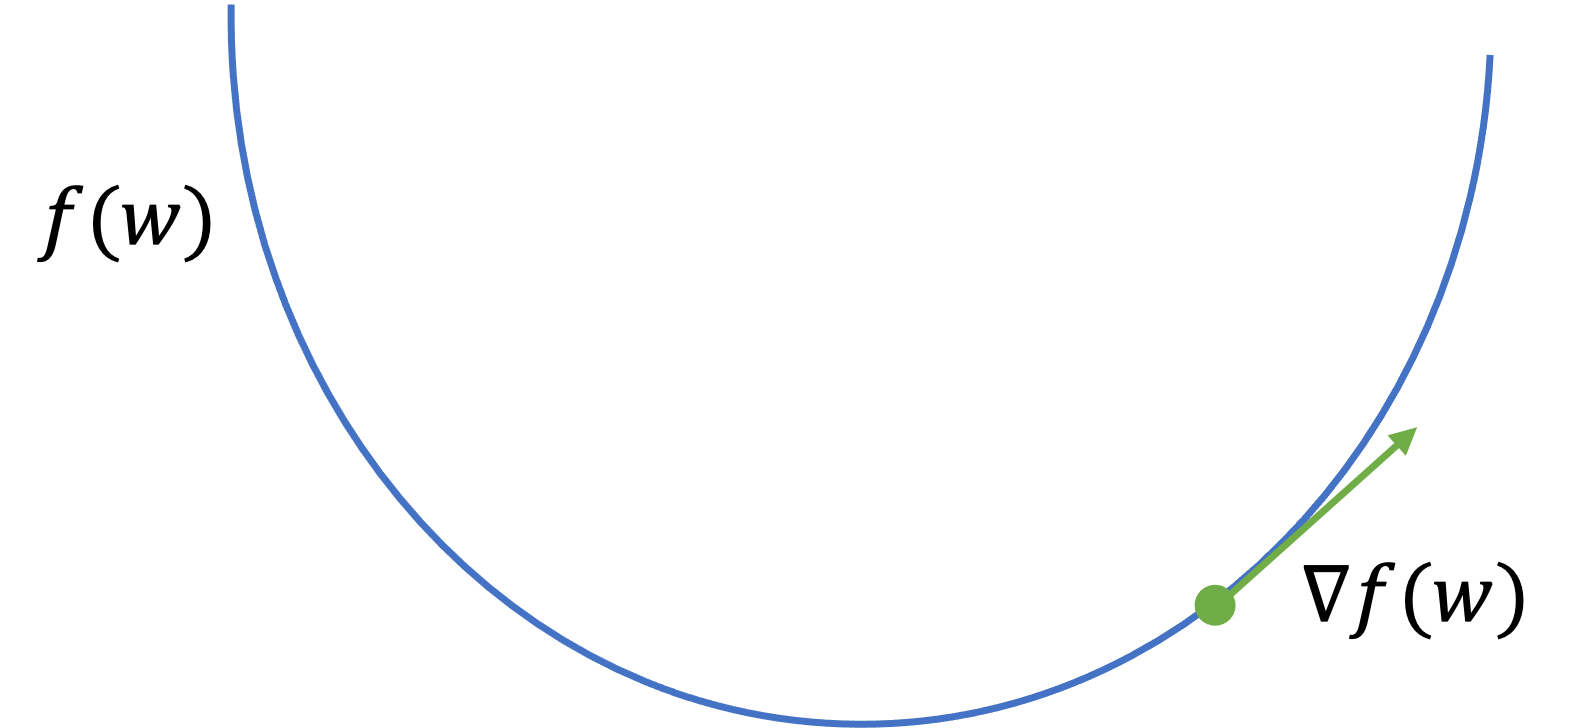
\includegraphics[width=0.5\textwidth]{geometric_gradient.png}
    \caption{Geometric gradient intuition.}
    \label{fig:geometric}
\end{figure}
From the graph of our convex function (Fig.~\ref{fig:geometric}), we can intuitively see that if one wants to find the minima of $f$, one must move in the opposite direction of the gradient. 
Thus, we can define the algorithm for gradient descent as follows:
\begin{algorithm}[!h]
\caption{Gradient Descent(f)}
\begin{algorithmic}[1]
\STATE $w^0 \gets 0$
\FOR{$t=1,...,T$}
    \STATE \texttt{COMPUTE}$(\nabla f(w^{t-1}))$
    \STATE $w^t \gets w^{t-1} - \eta \nabla f(w^{t-1})$ 
\ENDFOR
\end{algorithmic}
\end{algorithm}
In the above algorithm, we used our intuition about the geometry to define the update step in line 4. We move each weight in the direction of the negative gradient. The magnitude that we move is scaled by our learning rate $\nabla$. Later, we will see how careful tuning of $\nabla$ will affect the regret.

\subsection{Linear Approximation with Regularization Perspective}
In order to add some rigor to our intuition about the gradient update, let us explore gradient descent from the perspective of linear approximation with regularization.
\begin{figure}[!h]
    \centering
    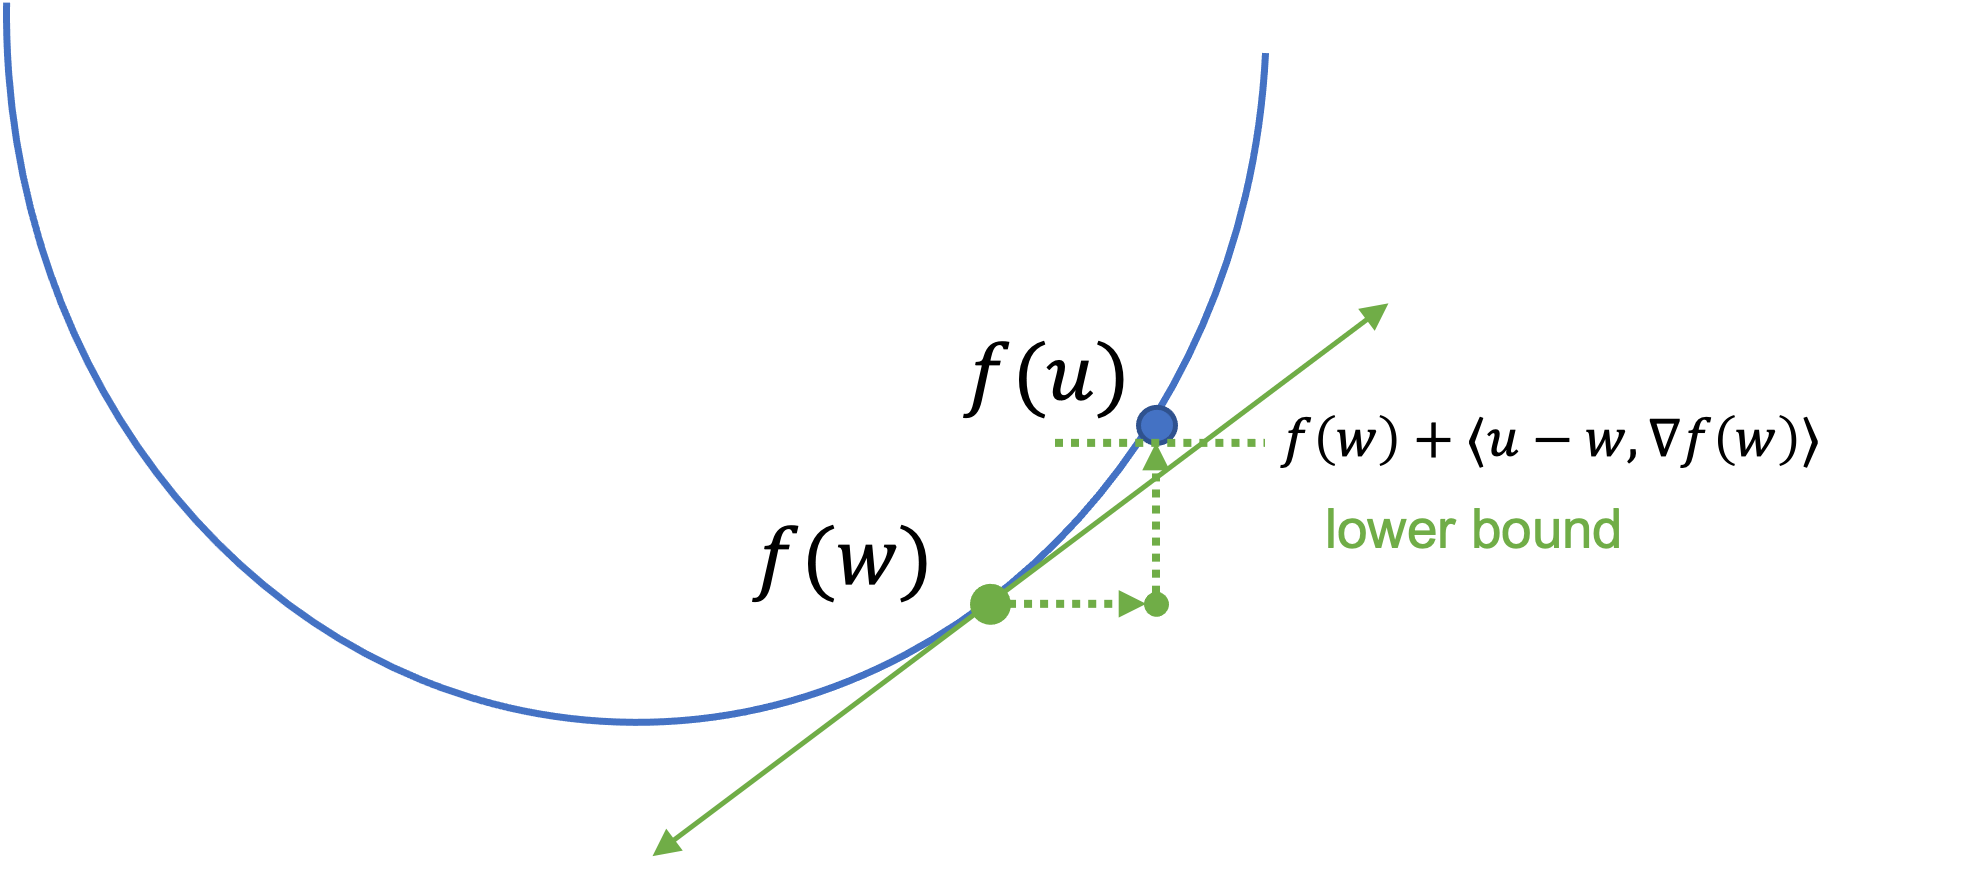
\includegraphics[width=0.5\textwidth]{regularized_gradient.png}
    \caption{Showing the lower bound of the first-order Taylor series approximation.}
    \label{fig:regularized}
\end{figure}
By taking a first-order Taylor series expansion of $f$ around $w$, we can approximate the value at some point $u$, $f(u) \approx f(w) + \langle u-w, \nabla f(w)\rangle$. 
\begin{lemma}
When $f$ is convex, the first-order Taylor series approximation is a lower bound.
\end{lemma}
Given the preceding lemma, we know, $f(u) \geq f(w) + \langle u-w, \nabla f(w)\rangle$. See Fig.~\ref{fig:regularized}.

One may think that we can minimize this approximation, $\min_u \{f(w) + (u-w)^\intercal \nabla f(w)\}$, directly, but this will result in a solution at negative infinity.

Recall that linear approximations are only accurate for values 'close to' $w$ ($\epsilon$-neighborhood). We can introduce a regularization term to the objective function to constrain the expression and express closeness. One such constraint is the squared L2 norm, $\min_w||w-w^t||^2_2$. Thus, our final objective function becomes a linear loss function with a quadratic regularization term:
$$w^{t+1} = \arg \min_w \frac{1}{2}||w-w^t||^2+\eta \big{(}f(w^t)+\langle w-w^t,\nabla f(w^t)\rangle\big{)}
$$
The first term in the objective function's purpose is regularization to keep the $w$ values close to $w^{t}$. At the same time, the second term in the objective function looks to find the minimum $w$ with respect to minimizing the approximation of $f$. The $\eta$, which we traditionally think of as our learning rate, is set up as the Lagrange multiplier in this dual objective optimization problem.

By taking the derivative of the objective function and setting it equal to 0, we can solve for $w^{t+1}$, deriving the gradient update step, $w^{t+1} = w^t - \eta \nabla f(w^t)$.

\subsection{Isometric Quadratic Approximation Perspective}
We know that online mirror descent can be used to solve functions with linear loss and quadratic regularization, so we need to analyze another perspective.
\begin{figure}[!h]
    \centering
    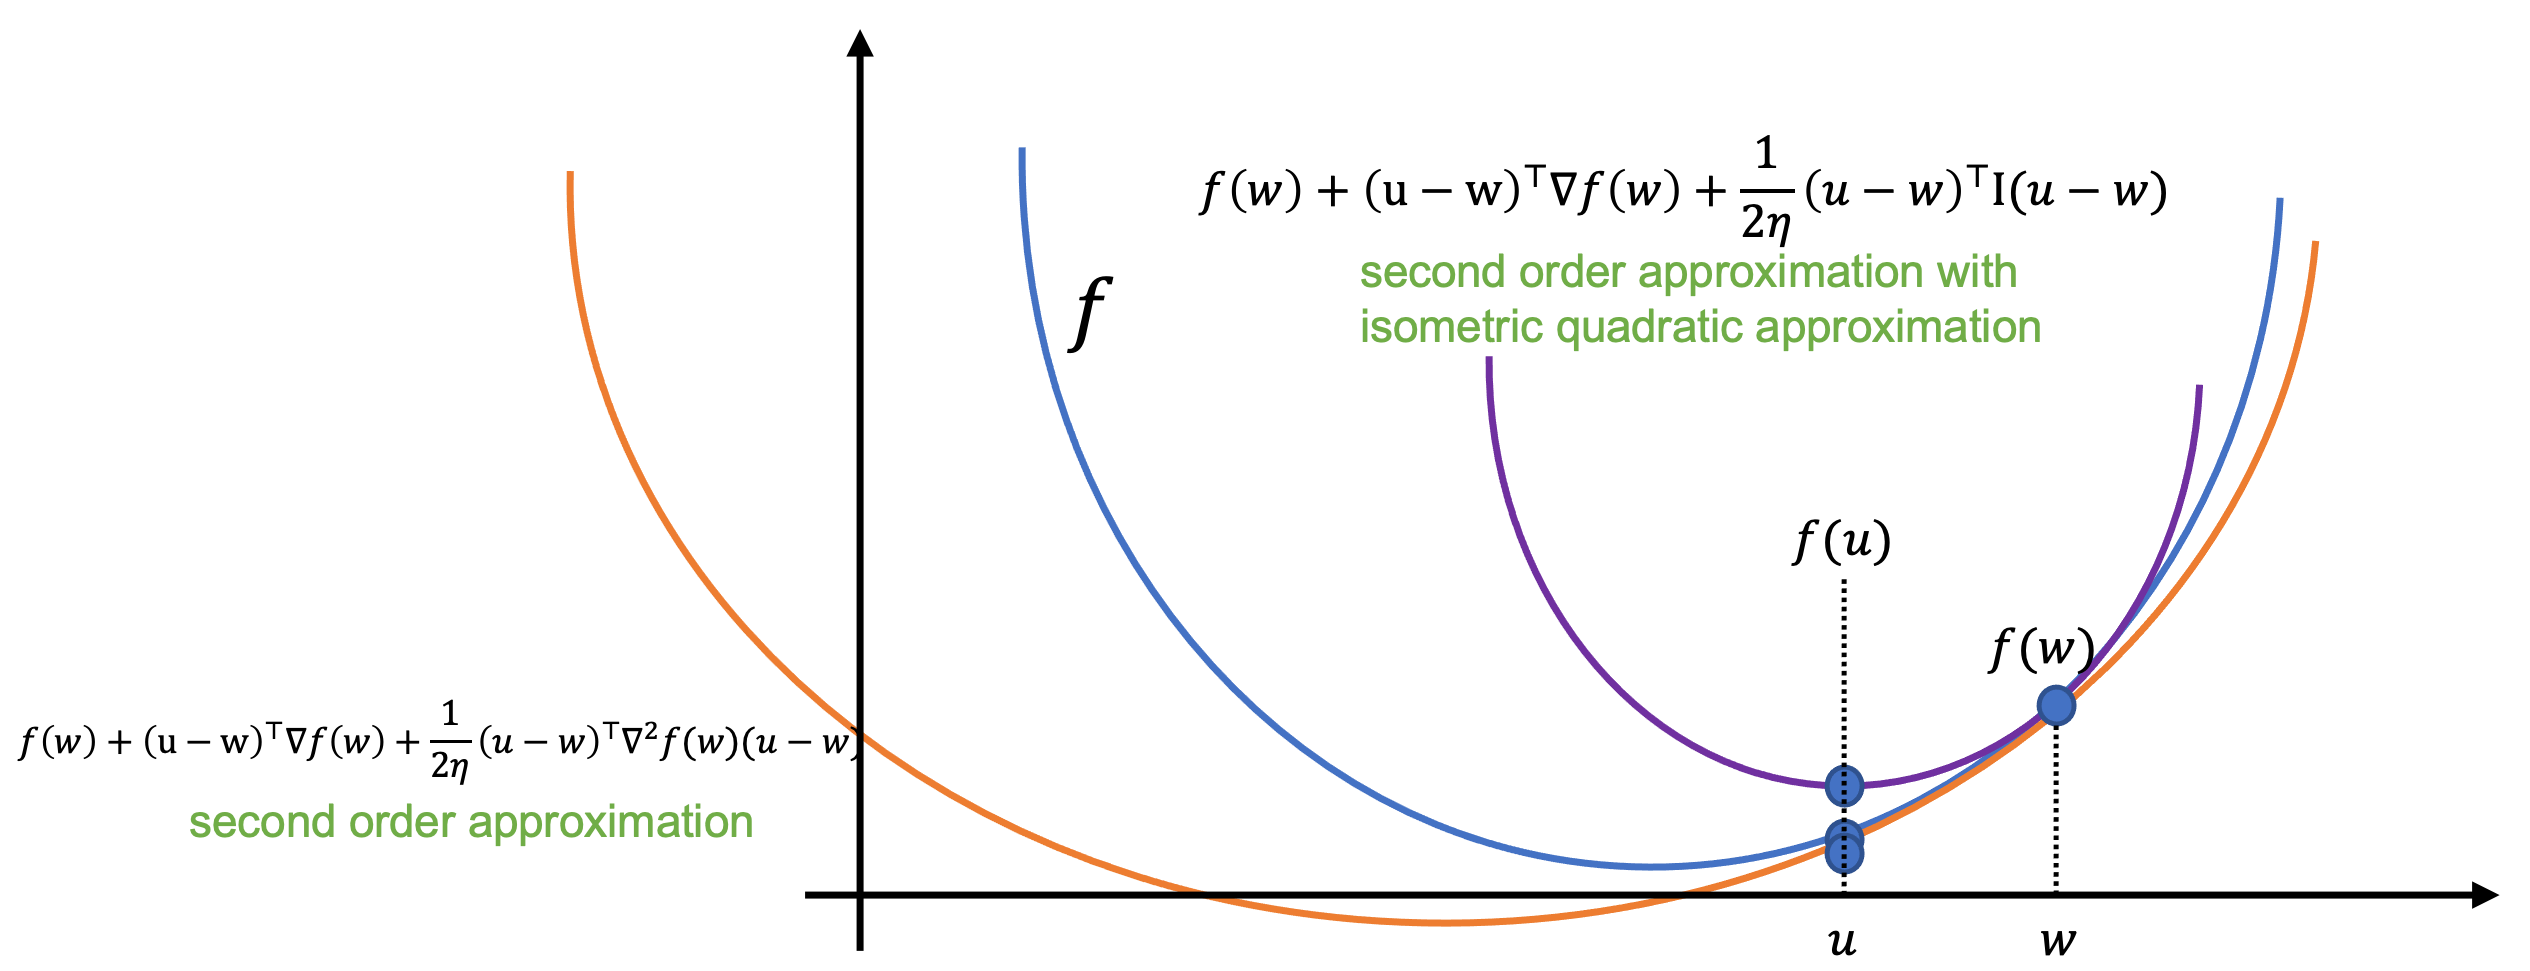
\includegraphics[width=0.75\textwidth]{isometric_gradient.png}
    \caption{The isometric approximation is shown above, compared to the original function and the second-order approximation.}
    \label{fig:isometric}
\end{figure}

A second-order Taylor expansion yields,
$$
    f(u) \approx f(w) + (u-w)^\intercal \nabla f(w) + \frac{1}{2}(u-w)^\intercal \nabla^2 f(w) (u-w).
$$
We can add a tunable scaling parameter to the second-order term and use an isometric quadratic approximation, i.e., unit scaling in all dimensions/directions, to get,
$$
    f(u) \approx f(w) + (u-w)^\intercal \nabla f(w) + \frac{1}{2\eta}(u-w)^\intercal \mathbf{I} (u-w).
$$
By multiplying the RHS by $\eta$ and rearranging the terms, we have derived the same objective function as before,
$$
w^{t+1} = \arg \min_w \frac{1}{2}||w-w^t||^2+\eta \big{(}f(w^t)+\langle w-w^t,\nabla f(w^t)\rangle\big{)}
$$
Similarly, we can take the derivative of the objective function and set it equal to 0. 
$$
\frac{\partial}{\partial w} \Big{\{} \frac{1}{2}||w-w^t||^2 + \eta \Big{(} f(w^t) +\langle w-w^t, \nabla f(w^t) \rangle \Big{)} \Big{\}} = 0
$$
$$
\frac{1}{2} \Big{(} 2w + 0 -2w^t\Big{)} + \eta \Big{(} 0 + \nabla f (w^t) - 0\Big{)} = 0
$$
$$
w - w^t + \eta \nabla f(w^t) = 0
$$
Then solve for $w$ to derive the gradient update step,
$$
w = w^t - \eta \nabla f(w^t),
$$
which we can use for $w^{t+1} = w^t - \eta \nabla f(w^t)$.

\subsection{Summary}
We have shown that we can find the parameter update, $$w^{t+1} = w^t - \eta \nabla f(w^t),$$
as a result of:
\begin{enumerate}
    \item a quadratic approximation of the loss function $f$
    \item a linear loss function $f$ with quadratic regularization
    \item a quadratic loss function with linear constraints
\end{enumerate}
Item 3 will be seen in the next lecture.

\section{OGD/SGD vs. OMD}
In this section, we will show how online gradient descent (OGD) may be equivalent to stochastic gradient descent (SGD) and how they are a special case of online mirror descent (OMD)~\cite{mcmahan2011follow}.
\subsection{Stochastic Gradient Descent}
We can speed up online gradient descent through stochastic gradient descent. Stochastic gradient descent is a convex optimizer which does not require the exact gradient. The direction of the descent will be a random vector. SGD only requires that the expected value at each iteration will equal the gradient direction. 

\begin{algorithm}[!h]
\caption{Stochastic Gradient Descent(f)}
\begin{algorithmic}[1]
    \STATE $w^1 \gets 0$
    \STATE $\eta > 0$
    \FOR{$t=1,...,T$}
        \STATE $z \sim D$
        \STATE $v^t = \nabla f_z (w^{t-1})$
        \STATE $w^t = w^{t-1} - \eta v^t$
    \ENDFOR
\end{algorithmic}
\end{algorithm}

We detail the stochastic gradient descent algorithm above. In line 4, the algorithm samples from the data distribution, which can be a single sample or a mini-batch. In line 5, we can quickly compute the gradient of a single sample or mini-batch. Since the expectation is the true gradient, the algorithm still holds. One may recall that this looks exactly like the online learning algorithm without $x$, and this looks exactly like online convex optimization.

\subsection{Method Connections}
We can connect Online gradient descent (OGD) / stochastic gradient descent to be a special case of online mirror descent.
Define the regularization function as, $\phi(w) = \frac{1}{2\eta} ||w||^2_2$, which is quadratic. Define the loss function as, $f(w) = \langle w, \theta \rangle$, which is linear. Then the prediction rule becomes,
$$
w^t+1 = \arg \min_w \langle w, -\theta^{t+1} \rangle + \phi(w).
$$
Substituting in our regularization function, we have,
$$
w^t+1 = \arg \min_w \langle w, -\theta^{t+1} \rangle + \frac{1}{2\eta} ||w||^2_2.
$$
For this combination, we can derive the analytical solution.
$$
w^t+1 = \arg \min_w \langle w, -\theta^{t+1} \rangle + \frac{1}{2\eta} \sqrt{\sum_n w^2_n}^2
$$
This is equivalent to,
$$
w^t+1 = \arg \min_w \langle w, -\theta^{t+1} \rangle + \frac{1}{2\eta} \sum_n w^2_n.
$$
Define, $\mathbf{L} = \langle w, -\theta^{t+1} \rangle + \frac{1}{2\eta} \sum_n w^2_n$.
We can take the derivative with respect to $w_n$ to find the minima,
$$
\frac{\partial \mathbf{L}}{\partial w_n} = -\theta_n + \frac{1}{2\eta} 2 w_n = 0.
$$
Thus, we have found the optimal parameter, $w_n = \eta \theta_n$, which is also a mapping from the dual parameter to the primal parameter. That is, we have found the mirror function for OGD, $g(\theta) = \eta \theta$.

We know that there are two versions of the OGD mirror function. The first is,
$$
g(\theta) = \Pi_{\theta \to S}(n\theta),
$$
which is a projection to the convex set. See algorithm \ref{alg:OPSGS} line 2 for the dual parameter update and line 3 for the mirror projection with some explicit condition on the feasibility set via projection.
The other is,
$$
\Pi_{x \to S}(x) = \arg \min_y ||x-y||^2,
$$
which, for example, is a euclidean projection to S. We found,
$$
g(\theta) = \eta \theta,
$$
which has no projection. This assumes a constrained range of sub-gradients, which will slightly change the regret analysis. See algorithm \ref{alg:OSGS} line 2 for the dual parameter update and assumption on the magnitude of the sub-gradient and line 3 for the mirror projection.

\begin{algorithm}
\caption{Online Sub-Gradient Descent($\eta$)}
\label{alg:OSGS}
\begin{algorithmic}[1]
    \FOR{$t=1,...,T$}
        \STATE $\theta^{t+1} = \theta^t - z^t$, $z^t \in \partial f^t(w^t)$
        \STATE $w^{t+1} = \eta \theta^{t+1}$
    \ENDFOR
\end{algorithmic}
\end{algorithm}

\begin{algorithm}
\caption{Online Proj Sub-Gradient Descent($\eta$)}
\label{alg:OPSGS}
\begin{algorithmic}[1]
    \FOR{$t=1,...,T$}
        \STATE $\theta^{t+1} = \theta^t - z^t$, $z^t \in \partial f^t(w^t)$
        \STATE $w^{t+1} = \Pi_{\theta \to S} \eta \theta^{t+1}$
    \ENDFOR
\end{algorithmic}
\end{algorithm}

Thus, we have shown that OGD is OMD with a linear loss and quadratic regularization (or quadratic loss and linear constraints).

\subsubsection{Quick Aside to Other Algorithms}
We can quickly see that this is similar to the perceptron algorithm with the following derivation.
From $$ w^{t+1} = \eta \theta^{t+1},$$ we expand the mirror function,
$
w^{t+1} = -\eta \sum_{i=1}^t z^i.
$
Separating the sum, we have,
$
w^{t+1} = -\eta (z^t + \sum_{i=1}^{t-1} z^i).
$
We can convert this to shorthand notation,
$
w^{t+1} = -\eta (z^t + \theta^t).
$
By definition of the weight vector,
$
w^{t+1} = -\eta (z^t - \frac{1}{\eta} w^t).
$
Then finally simplifying,
$
w^{t+1} = w^t - \eta z^t.
$


\section{Online Gradient Descent Analysis}
To begin the analysis of OGD, we first start with the general regret bound derived for OMD as shown below.
\[ R(u) = \sum_{t=1}^T (w^t \cdot z^t - u \cdot z^t) \leq \psi(u) - \psi(w^1) + \sum_{t=1}^T D_{\psi^*}(-z^{1:t}||-z^{1:t-1}) \]
The regularization function is defined as $\psi(w) = \frac{1}{2}||w||_2^2$. From this, we can derive that the convex conjugate can be defined as $\psi^*(\theta) = \frac{1}{2}||\theta||_2^2$. To do so, we first start with the convex conjugate definition and rearrange the terms as shown below.
\[ \psi^*(\theta) = \max_w (\langle \theta, w \rangle - \psi(w)) = -\min_w (\psi(w) - \langle \theta, w \rangle) \]
\[ \psi^*(\theta) = -\min_w (\frac{1}{2}||w||_2^2 - \langle \theta, w \rangle) \]
Next, we solve for the minima by finding for what $w$ the first-order optimality conditions are satisfied, as shown below.
\[ \frac{\partial}{\partial w}\{ \frac{1}{2}||w||_2^2 - \langle \theta, w \rangle) \} = 0 \]
\[ w - \theta = 0 \]
\[ w = \theta \]
Now, we revisit the original inequality $\psi^*(\theta) = -\min_w (\frac{1}{2}||w||_2^2 - \langle \theta, w \rangle)$ and rearrange the terms to derive the desired result as shown below.
\[ \psi^*(\theta) = -\min_w (\frac{1}{2}||w||_2^2 - \langle \theta, w \rangle) \]
\[ -\psi^*(\theta) = (\frac{1}{2}||\theta||_2^2 - \langle \theta, \theta \rangle) \]
\[ -\psi^*(\theta) = (\frac{1}{2}||\theta||_2^2 - ||\theta||_2^2) \]
\[ -\psi^*(\theta) = -\frac{1}{2}||\theta||_2^2 \]
\[ \psi^*(\theta) = \frac{1}{2}||\theta||_2^2 \]
Now, we can return to the general regret bound derived for OMD and replace the Bregman Divergence term with its corresponding definition, as shown below.
\[ R(u) = \sum_{t=1}^T (w^t \cdot z^t - u \cdot z^t) \leq \psi(u) - \psi(w^1) + \sum_{t=1}^T \psi^*(\theta^{t+1}) - \psi^*(\theta^t) - \nabla \psi^*(\theta^t)(\theta^{t+1}-\theta^t) \]
Next, we apply the definition of $\psi$ and the derived $\psi^*$ from above as shown below.
\[ R(u) \leq \frac{1}{2\eta}||u||_2^2 -  \frac{1}{2\eta}||w^1||_2^2 + \sum_{t=1}^T \frac{1}{2\eta}||\theta^{t+1}||_2^2 - \frac{1}{2\eta}||\theta^t||_2^2 - \nabla \frac{1}{2\eta}||\theta^t||_2^2(\theta^{t+1}-\theta^t) \]
Next, we note that $\nabla \frac{1}{2\eta}||\theta^t||_2^2 = \frac{1}{\eta}\theta^t$, so we can replace the term $\nabla \frac{1}{2\eta}||\theta^t||_2^2$ as shown below
\[ R(u) \leq \frac{1}{2\eta}||u||_2^2 -  \frac{1}{2\eta}||w^1||_2^2 + \sum_{t=1}^T \frac{1}{2\eta}||\theta^{t+1}||_2^2 - \frac{1}{2\eta}||\theta^t||_2^2 - \frac{1}{\eta}\theta^t(\theta^{t+1}-\theta^t) \]
Next, we note that $\frac{1}{2\eta}||\theta^{t+1}||_2^2 - \frac{1}{2\eta}||\theta^t||_2^2 - \frac{1}{\eta}\theta^t(\theta^{t+1}-\theta^t) = \frac{1}{2\eta}||\theta^{t+1} - \theta^t||_2^2$ by completing the square. Thus, we can replace the terms within the summation with the completed square term, as shown below.
\[ R(u) \leq \frac{1}{2\eta}||u||_2^2 -  \frac{1}{2\eta}||w^1||_2^2 + \sum_{t=1}^T \frac{1}{2\eta}||\theta^{t+1} - \theta^t||_2^2 \]
Next, using the incremental update definition $\theta^{t+1} = \theta^{t} - \eta z^{t}$, we can replace $\theta^{t+1}$ in the expression as shown below.
\[ R(u) \leq \frac{1}{2\eta}||u||_2^2 -  \frac{1}{2\eta}||w^1||_2^2 + \sum_{t=1}^T \frac{1}{2\eta}||\theta^{t} - \eta z^{t} - \theta^t||_2^2 = \frac{1}{2\eta}||u||_2^2 -  \frac{1}{2\eta}||w^1||_2^2 + \sum_{t=1}^T \frac{1}{2\eta}||-\eta z^{t}||_2^2 \]
Since $-\eta$ is a constant, it can be moved to the outside of the norm as $|\eta|^2$ as shown below.
\[ R(u) \leq \frac{1}{2\eta}||u||_2^2 -  \frac{1}{2\eta}||w^1||_2^2 + \sum_{t=1}^T \frac{\eta}{2}||z^{t}||_2^2 \]
Finally, since $\frac{1}{2\eta}||w^1||_2^2$ is always positive, we can remove it to derive a larger upper bound as shown below.
\[ R(u) \leq \frac{1}{2\eta}||u||_2^2 -  \frac{1}{2\eta}||w^1||_2^2 + \sum_{t=1}^T \frac{\eta}{2}||z^{t}||_2^2 \leq \frac{1}{2\eta}||u||_2^2 +  \sum_{t=1}^T \frac{\eta}{2}||z^{t}||_2^2 \]
\[ R(u) \leq \frac{1}{2\eta}||u||_2^2 +  \sum_{t=1}^T \frac{\eta}{2}||z^{t}||_2^2 \]
We define $D = \max ||u||_2 : u \in S$ as the maximum magnitude of the primal parameter. Furthermore, we define $G = \max ||z||_2 : z \in \partial f(w)$ as the maximum magnitude of the sub-gradient. We can use these to express the above bound as shown below.
\[ R(u) \leq \frac{1}{2\eta}||u||_2^2 +  \sum_{t=1}^T \frac{\eta}{2}||z^{t}||_2^2 \leq \frac{D^2}{2\eta} + \frac{\eta}{2}TG^2 \]
This is a general regret bound, but we can determine the regret bound for the optimal $\eta$ with respect to the above general regret bound. To do this, we compute the first order optimality conditions with respect to $\eta$ as shown below.
\[ \frac{\partial}{\partial \eta} (\frac{D^2}{2\eta} + \frac{\eta}{2}TG^2) = 0 \]
\[ -\frac{D^2}{2\eta^2} + \frac{TG^2}{2} = 0 \]
\[ \frac{D^2}{2\eta^2} = \frac{TG^2}{2} \]
\[ D^2 = \eta^2TG^2 \]
\[ \frac{D^2}{TG^2} = \eta^2 \]
\[ \eta = \sqrt{\frac{D^2}{TG^2}} = \frac{D}{G\sqrt{T}} \]
Note that since $\eta > 0$, we do not consider the negative root. Using this value of $\eta = \frac{D}{G\sqrt{T}}$, we can compute the regret bound as shown below.
\[ R(u) \leq \frac{D^2}{2\eta} + \frac{\eta}{2}TG^2 \]
\[ R(u) \leq \frac{D^2}{2\frac{D}{G\sqrt{T}}} + \frac{\frac{D}{G\sqrt{T}}}{2}TG^2 \]
\[  R(u) \leq DG\sqrt{T} \]
Thus, we have derived the regret bound for OGD as $R_{OGD} \leq DG\sqrt{T}$~\cite{zinkevich2003online}.


\section{Online Normalized Exponentiated Gradient Descent}
We note that the regularization function chosen above is not the only one we can choose. Suppose we choose to define the regularization function $\psi$ as negative entropy with respect to $w$. That is, we can define $\psi(w)$ as shown below.
\[ \psi(w) = \sum_{k=1}^K (w_k\log{w_k}) : w \in \mathbf{S}^K \]
Here, $\mathbf{S}^k$ is a K-simplex constraint, and negative entropy is convex. We can define the loss function as $f(w) = \langle w, \theta \rangle$, which is linear. The prediction rule can be represented as shown below.
\[ w^{t+1} = \arg\min_w \langle w, -\theta^{t+1} \rangle + \psi(w) \]
Replacing $\psi$ as the negative entropy with respect to $w$ and ensuring $w \in \mathbf{S}^K$ yields the following prediction rule.
\[ w^{t+1} = \arg\min_{w \in \mathbf{S}^K} \langle w, -\theta^{t+1} \rangle + \sum_{k=1}^K (w_k\log{w_k}) \]
We can migrate the simplex constraint to the objective to formulate a constrained Lagrange optimization function as shown below.
\[ w^{t+1} = \arg\min_{w} \langle w, -\theta^{t+1} \rangle + \sum_{k=1}^K (w_k\log{w_k}) + \lambda (1 - \sum_{k=1}^K w_k) \]
\[ \mathcal{L} = \langle w, -\theta^{t+1} \rangle + \frac{1}{\eta}\sum_{k=1}^K (w_k\log{w_k}) + \lambda (1 - \sum_{k=1}^K w_k) \]
We can solve the above constrained Lagrangian optimization problem by computing the first order necessary conditions for optimality, as shown below.
\[ \frac{\partial\mathcal{L}}{\partial w_n} = -\theta_n + \frac{1}{\eta}(1 + \log{w_n}) - \lambda = 0 \]
\[ \frac{1}{\eta}\log{w_n} = \theta_n - \frac{1}{\eta} + \lambda \]
\[ w_n = e^{\eta\theta_n - (1 - \eta\lambda)} = \frac{e^{\eta\theta_n}}{e^{(1 - \eta\lambda)}} \]

We can use the following mirror function,
$$
g(\theta) = \frac{\exp{(\eta \theta)}}{\sum_{n^\prime} \exp{(\eta \theta_{n^\prime})}}
$$

\begin{algorithm}
\caption{Online Norm-Exp\_GD($\eta$)}
\begin{algorithmic}[1]
    \FOR{$t=1,...,T$}
        \STATE $\theta^{t+1} = \theta^t = \eta z^t$, $z^t \in \partial f^t (w^t)$
        \STATE $w^{t+1} \propto \exp{(\eta \theta^{t+1})}$
    \ENDFOR
\end{algorithmic}
\end{algorithm}
Online Norm-Exp Gradient Descent (ONEGD) can be shown to derive the same update as the weighted majority algorithm.
From $$w_n^{t+1} = \frac{\exp{(\eta \theta_n^{t+1})}}{\sum_n^\prime \exp{(\theta_{n^\prime})}}$$
with some algebraic tricks, it is equivalent to,
$$
w_n^{t+1} = \frac{w_n^t \exp{(-\eta z_n^t)}}{\sum_k w_k^t \exp{(-\eta z_k^t)}}
$$
Thus, we have, 
$$
w_n^{t+1} \propto w_n^t \exp{(-\eta z_n^t)}
$$

The Hedge algorithm is an unnormalized exponentiated gradient descent algorithm.
\begin{algorithm}
\caption{Hedge Algorithm($\beta$)}
\begin{algorithmic}[1]
    \STATE $w^1 \gets \{w^1_n = 1\}^N_{n=1}$
    \FOR{$t=1,...,T$}
        \STATE \texttt{RECEIVE}($x^t \in \{-1,1\}$)
        \STATE $i \sim \texttt{MULTINOMIAL}(w^t / \Phi^t)$
        \STATE $\hat{y}^t = h_i(x^t)$
        \STATE \texttt{RECEIVE}($y^t \in \{-1,1\})$
        \STATE $w_n^{t+1} = w_n^t e^{\beta (1[y^t \neq h_n(x^t)])}$ $\forall n$
    \ENDFOR
\end{algorithmic}
\end{algorithm}
%\section*{References}
%Include your references here. Please cite any resources you found useful.	
%Populate the refs.bib file or list your references manually. Be consistent in formatting!
{
\bibliography{refs}
\bibliographystyle{abbrv}
}

%\section{Appendix}
%This section provides any relevant background material that was not covered in the lectures, but was found to be useful for understanding the material. 
%For example, derivations, theory underlying techniques employed, etc. 

%Additionally, this section can summarizes applications or extensions of these techniques found in the literature. 

\end{document} % Done!



